\documentclass{article}[18pt]
\usepackage{../../../../../format}
\lhead{CSys - OS}


\begin{document}
\begin{center}
\underline{\huge File System Implementation}
\end{center}
\section*{Take a shot every time you see 'block'}
\section{File-System Structure}
\begin{itemize}
	\item File Structure
	\begin{itemize}
		\item Logical Storage Unit
		\item Collection of related information
	\end{itemize}
	\item File system resides on secondary storage (disks)
	\begin{itemize}
		\item Provided user interface to storage, mapping logical to physical
		\item Provides efficient and convenient access to disk by allowing data to be stored, located retrived easily
	\end{itemize}
	\item Disk provides in-place rewrite and random access
	\begin{itemize}
		\item I/O transfers performed in \textbf{blocks} of \textbf{sectors} (usually 512 bytes)
	\end{itemize}
	\item File control block - storage structure consisting of information about a file
	\item Device driver controls the physical device
	\item File system organized into layers
\end{itemize}
\section{Layered File System}
\begin{center}
	Application Programs
\end{center}
$$\Downarrow$$
\begin{center}
	Logical File System
\end{center}
$$\Downarrow$$
\begin{center}
	File Organization Module
\end{center}
$$\Downarrow$$
\begin{center}
	Basic File System
\end{center}
$$\Downarrow$$
\begin{center}
	I/O System
\end{center}
$$\Downarrow$$
\begin{center}
	Devices
\end{center}
\section{File System Layers}
\begin{itemize}
	\item Device drivers manage I/O devices at the I/O control layer
	\item Basic file system given command like "retrieve block 123" translates to device driver
	\item Also manages memory buffers and caches (allocation, freeing, replacement)
	\begin{itemize}
		\item Buffers hold data in transit
		\item Caches hold frequently used data
	\end{itemize}
	\item File organisation module understands files, logical address, and physical blocks
	\begin{itemize}
		\item Translates logical block \# to physical block \#
		\item Manages free space, disk allocation
	\end{itemize}
	\item Logical file system manages metadata information
	\begin{itemize}
		\item Translates file name into file number, file handle, location by maintaining file control blocks
		\item Directory management
		\item Protection
	\end{itemize}
	\item Layering useful for reducing complexity and redundancy, but adds overhead and can decrease performance. Translates file name into file number, file handle, location by maintaining file control blocks
	\begin{itemize}
		\item Logical layers can be implemented by any coding method according to OS designer
	\end{itemize}
\end{itemize}
\section{File-System Implementation}
\begin{itemize}
	\item We have system calls at the API level, but how do we implement their functions
	\begin{itemize}
		\item On disk and in memory structures
	\end{itemize}
	\item Boot control block contains info needed by system to boot OS from that volume
	\begin{itemize}
		\item Needed if volume contains OS, usually the first block of the volume
	\end{itemize}
	\item Volume control block (superblock, master file table) contains volume details
	\begin{itemize}
		\item Total \# of blocks, \# of free blocks, block size, free block pointers or array
	\end{itemize}
	\item Directory structure organizes the files
	\begin{itemize}
		\item Names and inode numbers, master file table
	\end{itemize}
	\item Per-file \textbf{File Control Block (FCB)} contains many details about the file
	\begin{itemize}
		\item Inode number, permissions, size, dates
		\item NTFS stores into a master file table using relational DB structures
	\end{itemize}
\end{itemize}
\begin{center}
	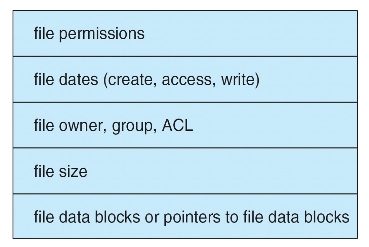
\includegraphics[scale=0.7]{Implementation}
\end{center}
\section{In-Memory File system structures}
\begin{itemize}
	\item Mount table storing file system mounts, mount points, file system types
	\item The following figure illustrates the necessary file system structures provided by the operating systems
	\item Figure (a) refers to opening a file
	\item Figure (b) refers to reading a file
	\item Plus buffers hold data blocks from secondary storage
	\item Open returns a file handle for subsequent use
	\item Data from read eventually copied to specified user process memory address
\end{itemize}
\begin{center}
	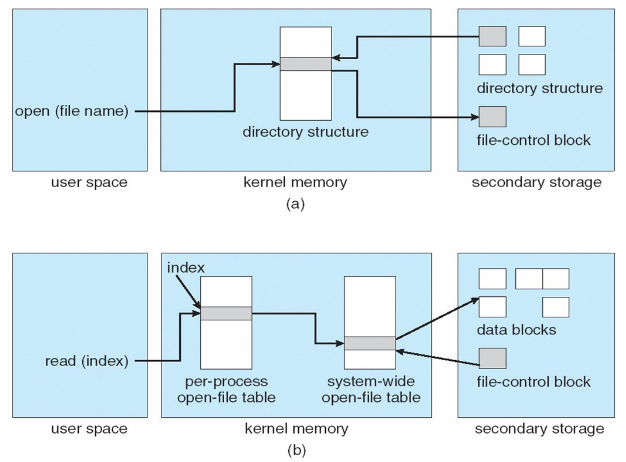
\includegraphics[scale=0.7]{Structure}
\end{center}
\section{Partitions and Mounting}
\begin{itemize}
	\item Partition can be a volume containing a file system ("cooked") or \textbf{raw} - just a sequence of blocks with no file system
	\item Boot block can point to boot volume or boot loader set of blocks that contain enough code to know how to load the kernel from the file system, or a boot management program for multi-os booting
	\item Root partition contains the OS, other partitions can hold other OSes, other file systems, or be raw
	\begin{itemize}
		\item Mounted at boot time
		\item Other partitions can mount automatically or manually
	\end{itemize} 
	\item At mount time, file system consistency is checked if the metadata is correct
	\begin{itemize}
		\item If not, fix it, try again
		\item If yes, add to mount table, allow access
	\end{itemize}
\end{itemize}
\section{Virtual File systems}
\begin{itemize}
	\item Virtual File Systems (VFS) on Unix provide an object-oriented way of implementing file systems
	\item VFS allows the same system call interface (the API) to be used for different types of file systems
	\begin{itemize}
		\item Separates file-system generic operations from implementation details
		\item Implementation can be one of many file systems types, or network file system
		\begin{itemize}
			\item Implements vnodes which hold inodes or network file details
		\end{itemize}
		\item Then dispatches operation to appropriate file system implementation routines
	\end{itemize}
	\item The API is to the VFS interface, rather than any specific type of file system
\end{itemize}
\begin{center}
	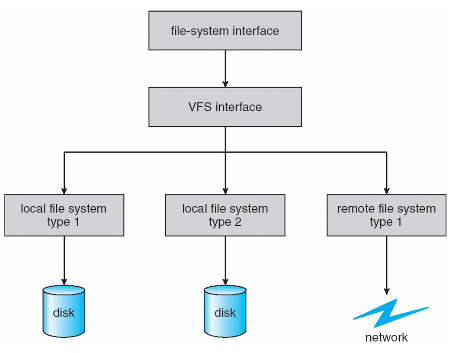
\includegraphics[scale=0.7]{VFS}
\end{center}
\section{Directory Implementation}
\begin{itemize}
	\item Linear list of file names with pointer to the data blocks
	\begin{itemize}
		\item Simple to program
		\item Time consuming to execute
		\begin{itemize}
			\item Linear search time
			\item Could keep ordered alphabetically via linked list or use B+ tree
		\end{itemize}
	\end{itemize}
	\item Hash table - linear list with hash data structure
	\begin{itemize}
		\item Decreases directory search time
		\item Collisions - situations where two file names hash to the same location
	\end{itemize}
\end{itemize}
\section{Allocation Methods - Contiguous}
\begin{itemize}
	\item An allocation method refers to how disk blocks are allocates for files
	\item Contiguous allocation - each file occupies set of contiguous blocks
	\begin{itemize}
		\item Best performance in most cases
		\item Simple - only starting location (block \#) and length (number of blocks) are required
		\item Problems include finding space for file, knowing file size, external fragmentqation, need for compaction off-line (downtime) or on-line
	\end{itemize}
	\item Mapping from logical to physical
\end{itemize}
\begin{center}
	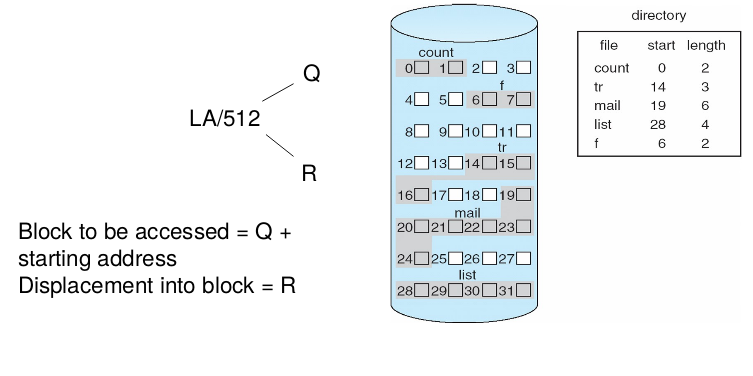
\includegraphics[scale=0.7]{Allocation}
\end{center}
\section{Extent-Based systems}
\begin{itemize}
	\item Many newer file systems (i.e., Veritas File System) use a modified contiguous allocation scheme
	\item Extent-based file systems allocate disk blocks in extents
	\item An extent is a contiguous chunk of blocks
	\begin{itemize}
		\item Extents are allocated for file allocation
		\item A file consists of one or more extents
	\end{itemize}
\end{itemize}
\section{Allocation methods - linked}
Linked allocation - each file a linked list of blocks
\begin{itemize}
	\item File ends at nil pointer
	\item No external fragmentation
	\item Each block contains pointer to next block
	\item No compaction, external fragmentation
	\item Free space management system called when new block needed
	\item Improve efficiency by clustering blocks into groups but increases internal fragmentation
	\item Reliability can be a problem
	\item Locating a block can take many I/Os and disk seeks
\end{itemize}
FAT (File Allocation Table) variation - CHONKY AF
\begin{itemize}
	\item Beginning of volume has table, indexed by block number
	\item Much like a linked list, but faster on disk and cacheable
	\item New block allocation simple
\end{itemize}
\section{Linked allocation}
Each file is a linked list of disk blocks: blocks may be scattered anywhere on the disk
\begin{center}
	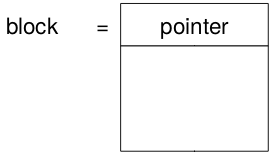
\includegraphics[scale=0.7]{Linked}
\end{center}
Mapping
\begin{center}
	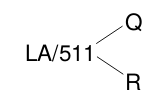
\includegraphics[scale=0.7]{Linked1}
\end{center}
Block to be accessed is the Qth block in the linked chain of blocks representing the file\\
Displacement into block $=R+1$
\begin{center}
	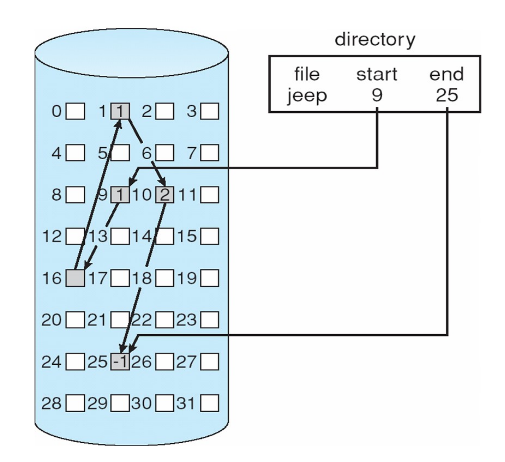
\includegraphics[scale=0.7]{Linked2}
\end{center}
\section{File-Allocation Table}
\begin{center}
	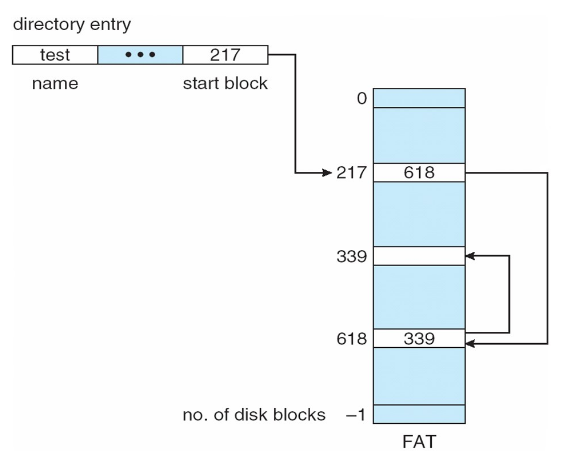
\includegraphics[scale=0.7]{FAT}
\end{center}
\section{Allocation Methods - Indexed}
Indexed allocation - each file has its own index block(s) of pointers to its data blocks\\
\\
Logical view
\begin{center}
	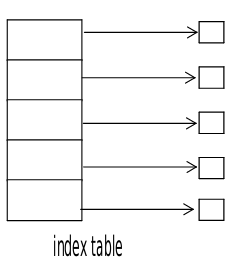
\includegraphics[scale=0.7]{index}
\end{center}
\begin{center}
	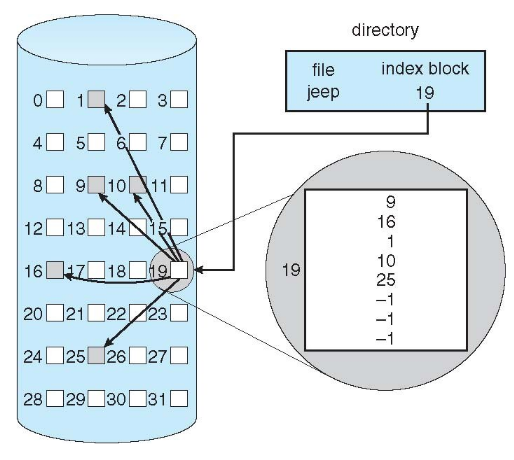
\includegraphics[scale=0.7]{index1}
\end{center}
\begin{itemize}
	\item Need index table
	\item Random access
	\item Dynamic access without external fragmentation, but have overhead of index block
	\item Mapping from logical to physical in a file of maximum size of 256K bytes and block size of 512 bytes. We need only 1 block for index table
\end{itemize}
\begin{center}
	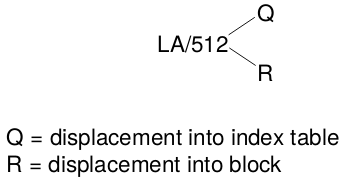
\includegraphics[scale=0.7]{index2}
\end{center}
\begin{itemize}
	\item Mapping from logical to physical in a file of unbounded length (block size of 512 words)
	\item Linked scheme - Link blocks of index table (no limit on size)
\end{itemize}
\begin{center}
	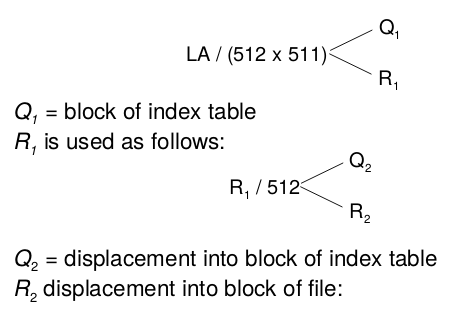
\includegraphics[scale=0.7]{index3}
\end{center}
\begin{itemize}
	\item Two-level index (4K blocks could store 1,024 four-byte pointers in outer index $\rightarrow$ 1,048,567 data blocks and file size of up to 4GB)
\end{itemize}
\begin{center}
	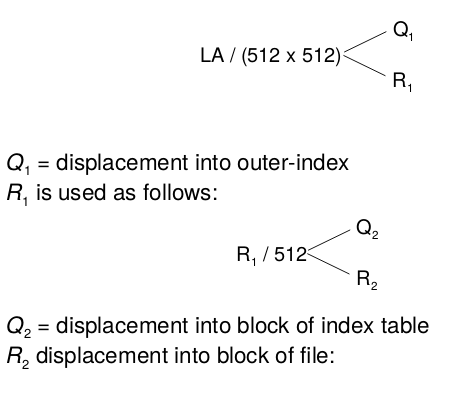
\includegraphics[scale=0.7]{index4}
\end{center}
\begin{center}
	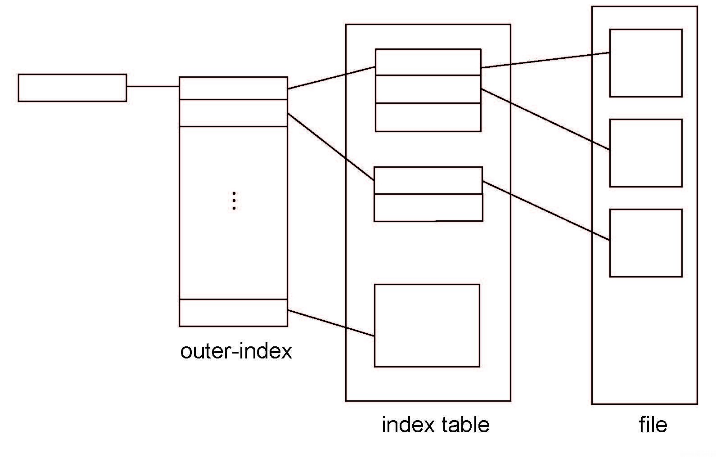
\includegraphics[scale=0.7]{index5}
\end{center}
\section{Combined Scheme: UNIX UFS}
4K bytes per block, 32-bit addresses
\begin{center}
	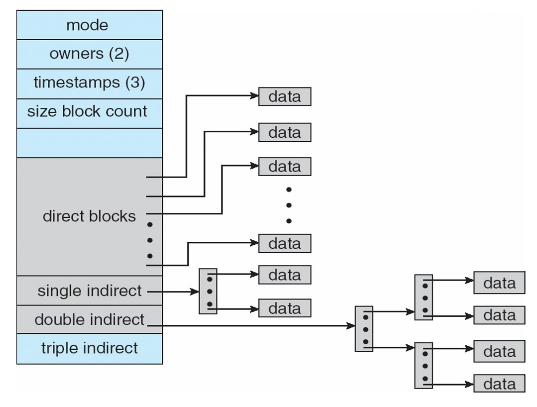
\includegraphics[scale=0.7]{UFS}
\end{center}
More index blocks than can be addressed with 32-bit file pointer
\section{Performance}
\begin{itemize}
	\item Best method depends on file access type
	\begin{itemize}
		\item Contiguous great for sequential and random
	\end{itemize}
	\item Linked good for sequential, not random
	\item Declare access type at creation $\rightarrow$ select either contiguous or linked
	\item Indexed more complex
	\begin{itemize}
		\item Single block access could require 2 index block reads then data block read
		\item Clustering can help improve throughput, reduce CPU overhead
	\end{itemize}
	\item Adding instructions to the execution path to save one disk I/O is reasonable
\end{itemize}
\section{Free space management}
\begin{itemize}
	\item Using term "block" for simplicity
	\item File system maintains free-space list to track available blocks/clusters
	\item Bit vector or bit map (n blocks)
\end{itemize}
\begin{center}
	\includegraphics[scale=0.7]{"Free Space"}
\end{center}
\begin{itemize}
	\item Bit map requires extra space
	\item Easy to get contiguous files
\end{itemize}
\section{Linked Free space list on disk}
Linked list (free list)
\begin{itemize}
	\item Cannot get contiguous space easily
	\item No waste of space
	\item No need to traverse the entire list (if \# of free blocks recorded)
\end{itemize}
\begin{center}
	\includegraphics[scale=0.7]{"Linked Free Space"}
\end{center}
\section{Efficiency and Performance}
Efficiency dependent on:
\begin{itemize}
	\item Disk allocation and directory algorithms
	\item Types of data kept in file's directory entry
	\item Pre-allocation or as-needed allocation of metadata structures
	\item Fixed-size or varying data structures
\end{itemize}
Performance
\begin{itemize}
	\item Keeping data and metadata close together
	\item Buffer cache - separate section of main memory for frequently used blocks
	\item Synchronous writes sometimes requested by apps or needed by OS
	\begin{itemize}
		\item No buffering/caching - writes must hit disk before acknowledgement
		\item Asynchronous writes more common, buffer-able, faster
	\end{itemize}
	\item Free-behind and read-ahead - techniques to optimize sequential access
	\item Reads slower than writes
\end{itemize}
\section{Recovery}
\begin{itemize}
	\item Consistency checking - compares data in directory structure with data blocks on disk, and tries to fix inconsistencies. Can be slow and sometimes fails
	\item Use system programs to back up data from disk to another storage device (magnetic tape, other magnetic disk, optical)
	\item Recover lost file or disk by restoring data from backup
\end{itemize}
\section{Log structured file systems}
\begin{itemize}
	\item Log structured (or Journaling) file systems record each metadata update to the file system as a transaction
	\item All transactions are written to a log
	\begin{itemize}
		\item A transaction is considered committed once it is written to the log (sequentially)
		\item Sometimes to a separate device or section of disk
		\item However, the file system may not be updated
	\end{itemize}
	\item The transactions in the log are asynchronously written to the file system structures
	\begin{itemize}
		\item When the file system strucrures are modified, the transaction is removed from the log
	\end{itemize}
	\item If the file system crashes, all remaining transactions in the log must still be performed
	\item Faster recovery from crash, removes chance of inconsistency of metadata
\end{itemize}
\end{document}